\hypertarget{Approach}{
}
In this section, the data and methods used for the experimental setup are outlined. Due to the unavailability of the ALOT database at the time of this research, only the PhoTex database is considered for the experiments. 

\section{PhoTex Database}\label{sec:PhoTex}
The PhoTex database is created for physics-based computer vision. It provides excellent photometric data for texture classification, since all image data is  created under controlled conditions. The materials were recorded under a fixed view and different illumination angles. It also provides the materials under a rotated angle, but these images are discarded for the experiments conducted in this research. The most important features of the database for this research are:

\begin{itemize}
	\item Images are monochromatic.
	\item Resolution: 512 x 512
	\item Fixed and linear gain: images measured under different lighting conditions are comparable. 
\end{itemize}

\noindent The database mainly holds images of rough surfaces, and a few smooth surfaces. For all the image data, the azimuth and zenith angles of the light source are provided (these angles are also mentioned as slant and tilt), making it perfect for photometric stereo algorithms to recover the surface normals and albedo of the materials. The general setup for recording the materials can be seen in figure \ref{fig:PHOTEX_SETUP}. 

Example images are shown in figure \ref{fig:PhoTexExamples} and give an indication of how much material can vary in appearance when observed from different illumination angles.

The images used in Targhi's experiment are chosen to have a high degree of diffuse reflection properties, since he only used the Lambertian reflectance model for image synthesis. In order to deal with possible illumination changes in both original and synthesized data, it is desirable to preprocess the images such that they are intensity invariant by setting the images to zero-mean and unit-variance. 

\begin{figure}[htbp!]
	\begin{center}
		\subfigure[aab]{
\epsfig{file=images/examples/0.aab.0.30.0.eps, width=0.15\linewidth}}
		\subfigure[acd]{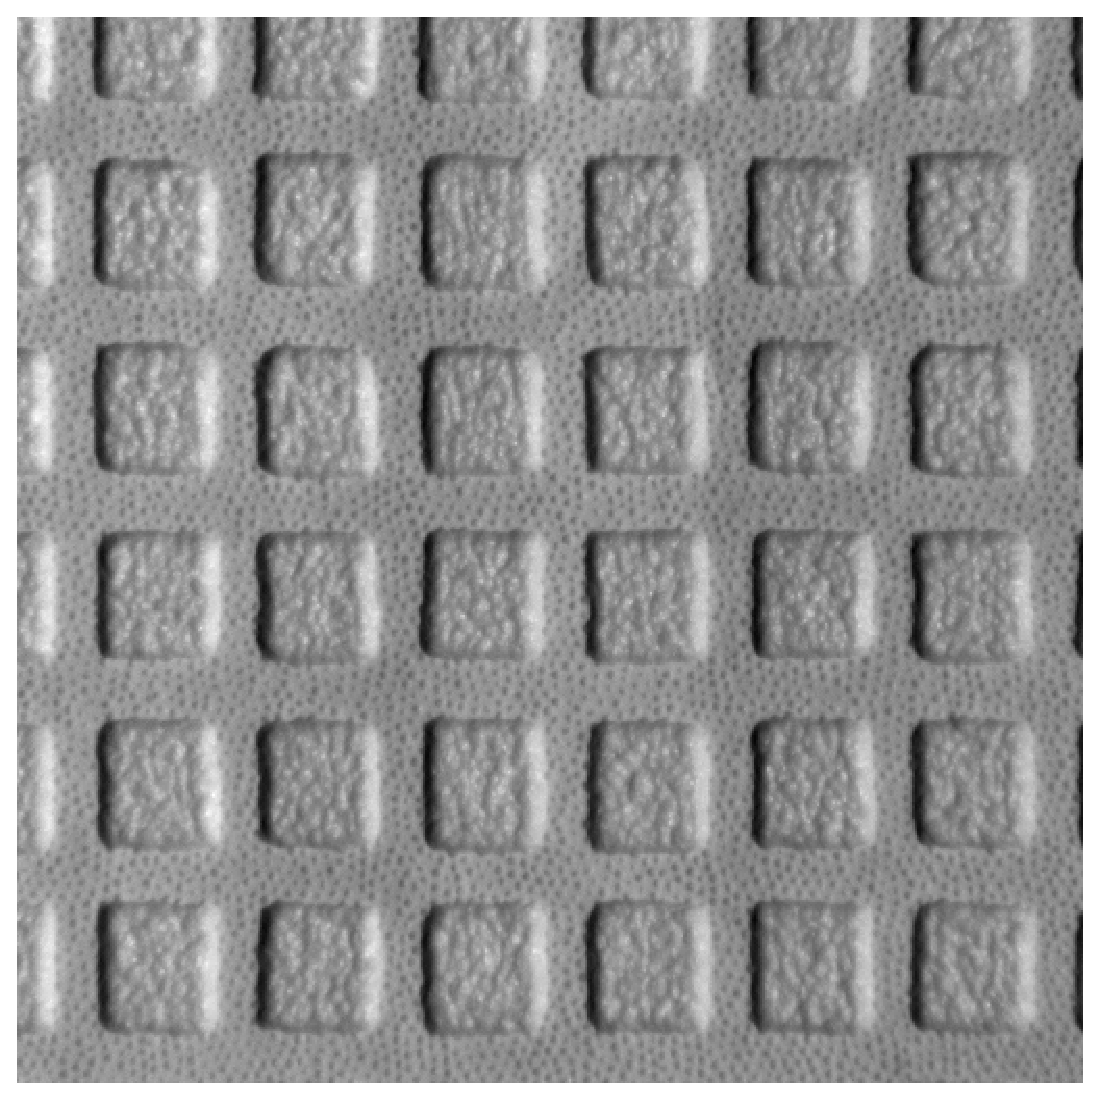
\epsfig{file=images/examples/1.acd.0.30.0.eps, width=0.15\linewidth}}
		\subfigure[adh]{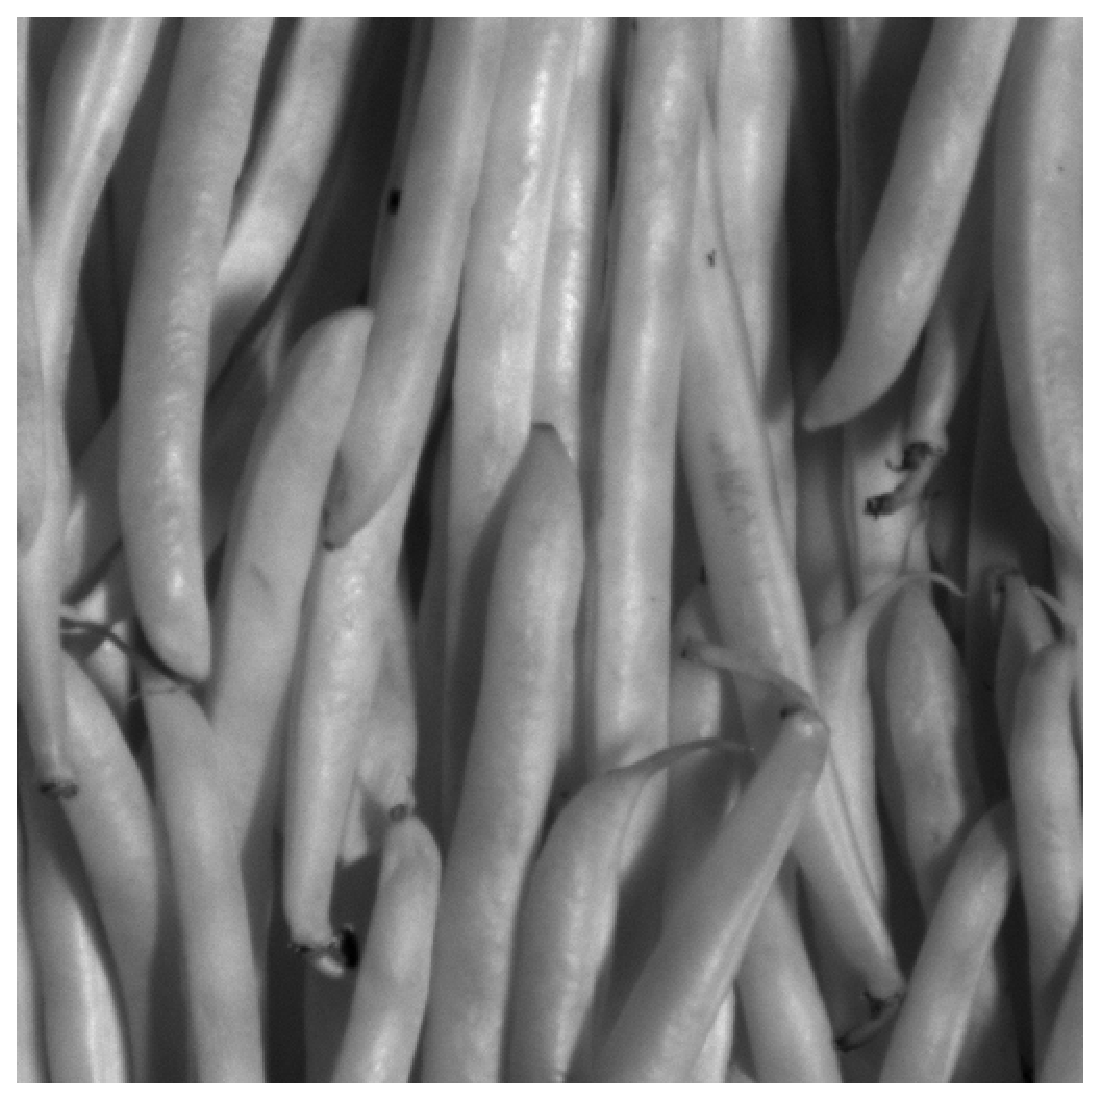
\epsfig{file=images/examples/2.adh.0.30.0.eps, width=0.15\linewidth}}

		\subfigure[aab]{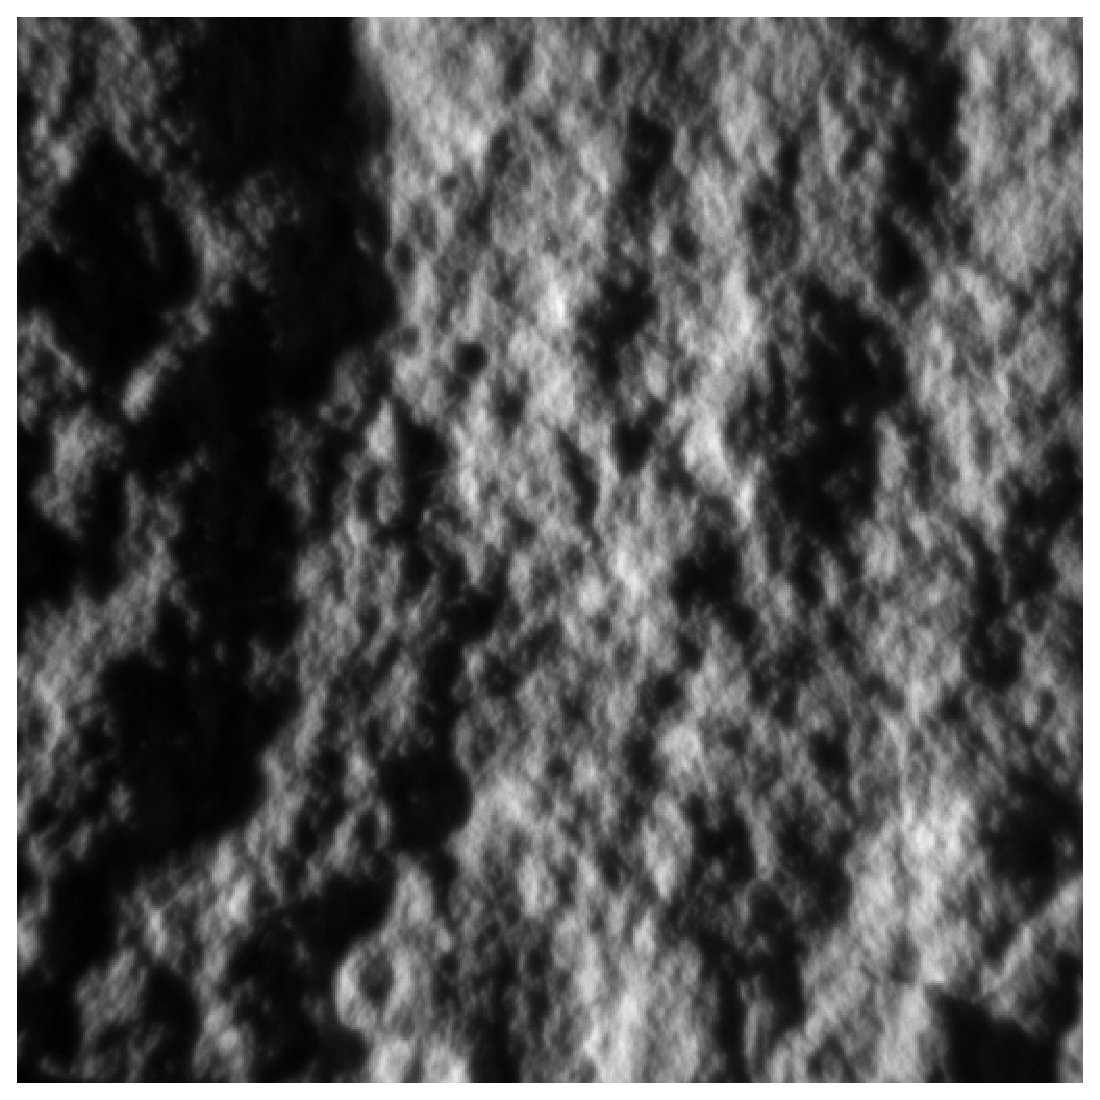
\epsfig{file=images/examples/0.aab.0.75.180.eps, width=0.15\linewidth}}
		\subfigure[acd]{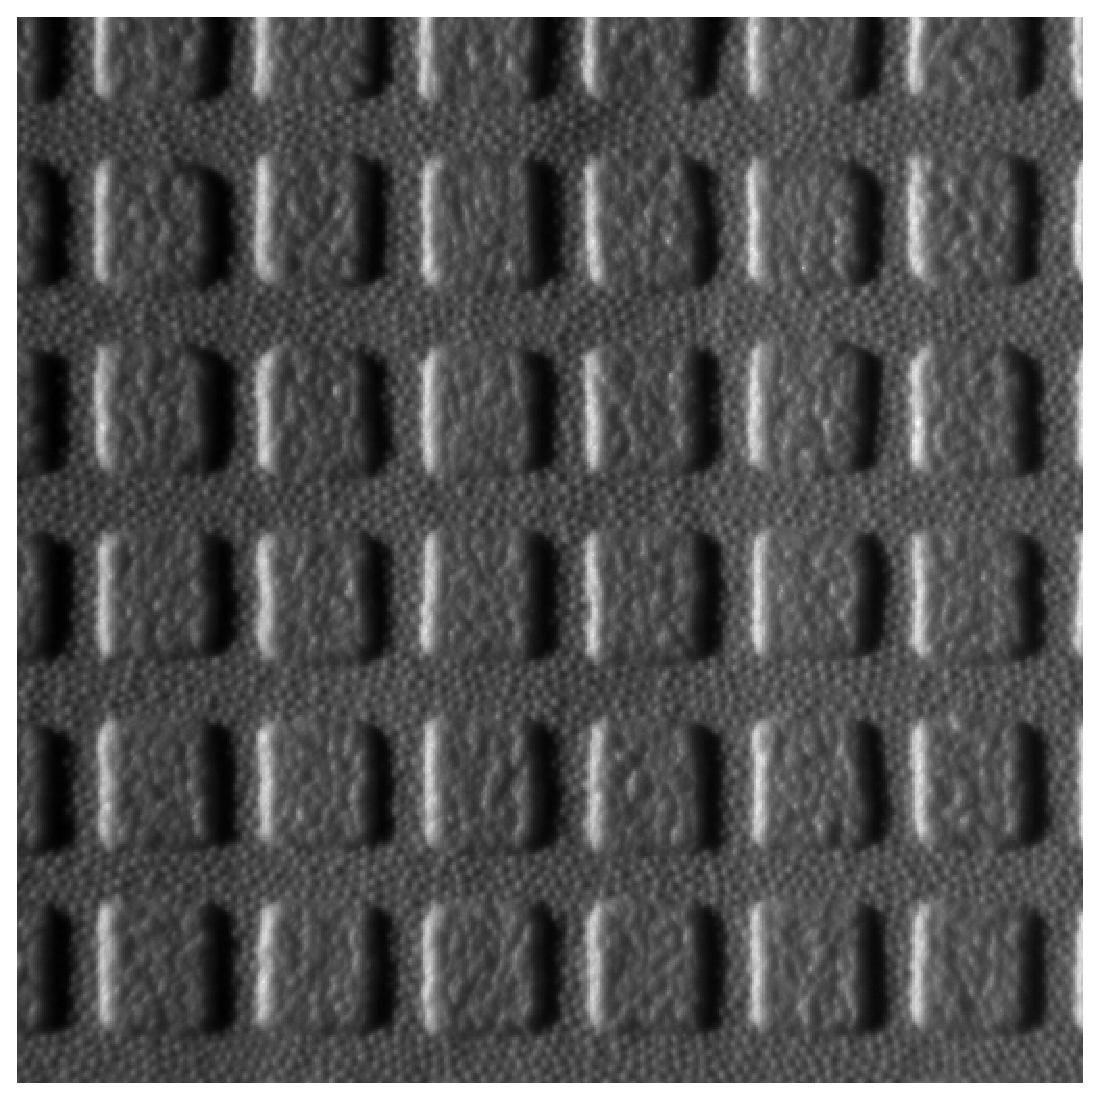
\epsfig{file=images/examples/1.acd.0.75.180.eps, width=0.15\linewidth}}
		\subfigure[adh]{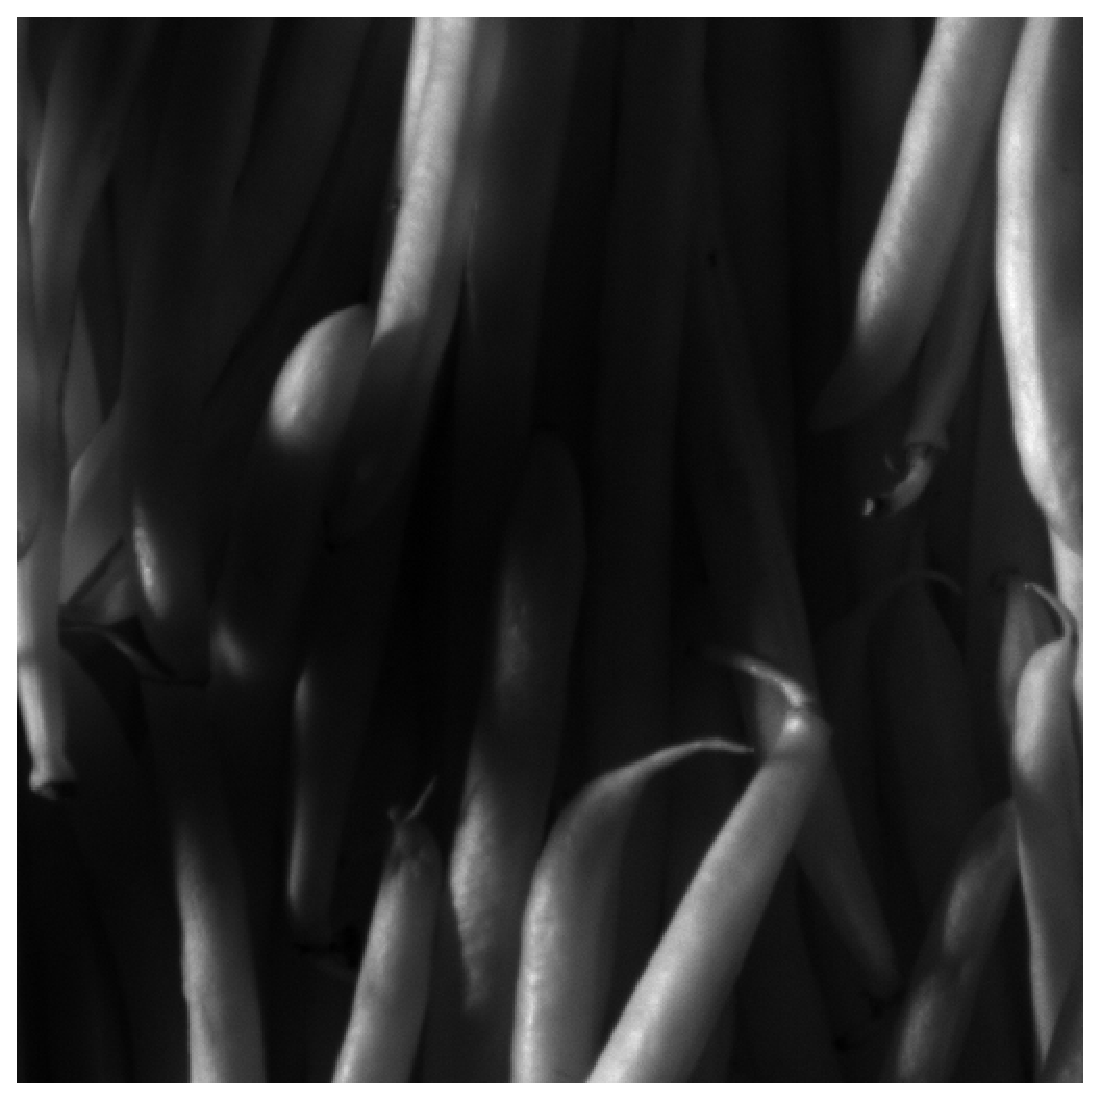
\epsfig{file=images/examples/2.adh.0.75.180.eps, width=0.15\linewidth}}
	\end{center}
	\caption{Example images from the PhoTex database. The upper row is recorded under a slant of $30^o$ and a tilt of $0^o$. The lower row is recorded under a slant of $75^o$ and a tilt of $180^o$.}
	\label{fig:PhoTexExamples}
\end{figure}


\begin{figure}[htbp!]
	\begin{center}
		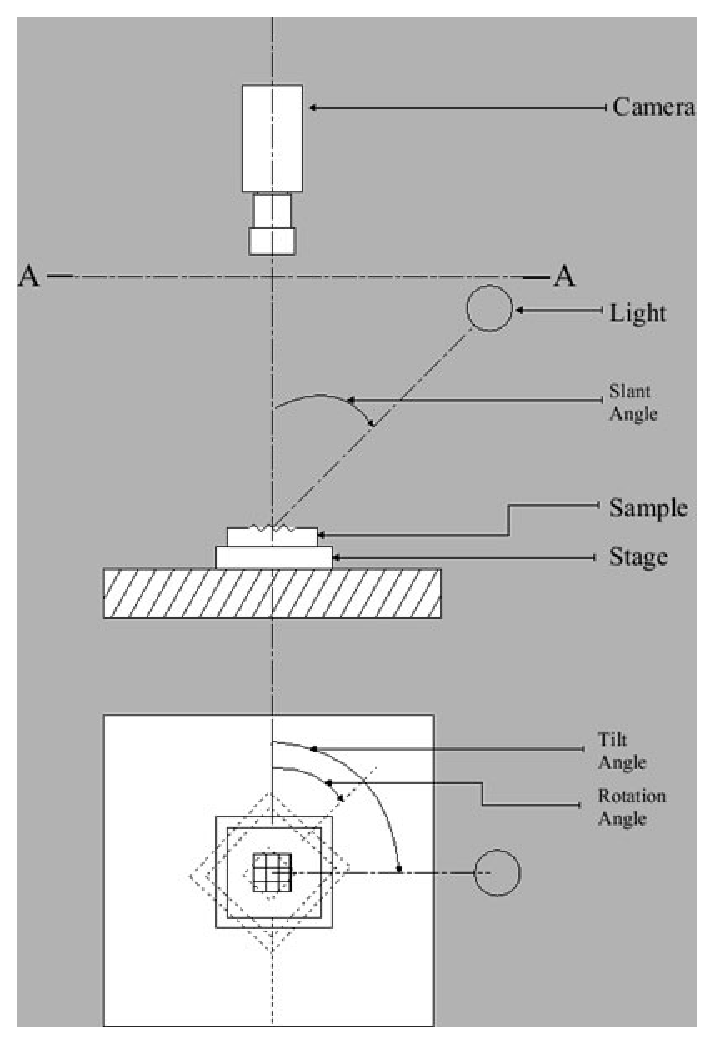
\epsfig{file=images/photex_setup.eps, width=0.5\linewidth}
	\end{center}
	\caption{\textit{Experimental setup of the recording of the PhoTex Database. Courtesy TextureLab @ Heriot-Watt University}}
	\label{fig:PHOTEX_SETUP}
\end{figure}

\section{Photometric Stereo}\label{sec:PhotometricStereo}
The aim of photometric stereo is to estimate at every point of a given object the albedo and surface normal. This is done by using a set of images of this object recorded under different illumination conditions. 

The viewpoint is assumed to be orthogonal to the surface patch that needs to be recovered, and the source light illuminating the surface patch is assumed to be a point light (\textit{eg.} the source is positioned at an infinite distance with as a result give an equal angle of incidence for all points on the surface patch). Using the assumption that the surface patch scatters light perfectly Lambertian and assuming there is no global illumination present in the data, the radiosity \textbf{B} at a point $(x, y)$ on the surface can be written as:

	\begin{eqnarray*}
		\textbf{B}(x,y) = \rho(x,y)\textbf{N}(x,y) \cdot \mathcal{V}
	\end{eqnarray*}

\noindent With $\rho(x,y)$ the albedo at point $(x,y)$, $\textbf{N}(x,y)$ being the surface normal at point $(x,y)$ and $\mathcal{V}$ being the source light vector. Both the surface normal and source light vector are unit in length. With the assumption that the camera response is linear to the surface radiosity, the value for a pixel at point $(x,y)$ in the image is equal to the radiance at that point. The above equation can be written as:

	\begin{eqnarray*}
		I(x,y) =  \textbf{g}(x,y) \cdot \mathcal{V}
	\end{eqnarray*}

\noindent Where $\textbf{g}(x,y)$ is equal to $\rho(x,y)\textbf{N}(x,y)$ and describes the properties of the surface we want to recover. Given that $\mathcal{V}$ is known for the image data, with enough dot products between $\textbf{g}(x,y)$ and $\mathcal{V}$, the values for $\textbf{g}$ could be recovered. With known values for $\textbf{g}$, the albedo and surface normals in turn could be recovered.

If we have $n$ images all recorded under the same viewing angle with $n$ different light sources with known light source direction, we can construct a matrix where all values $V_i$ are stacked on each other:

	\begin{eqnarray*}
		\mathcal{V} = \begin{pmatrix} V_1^T \\ V_2^T \\ ... \\ V_n^T \end{pmatrix}
	\end{eqnarray*}

\noindent Then, for each image point in our set of image data, the intensity values are stacked into a vector:

	\begin{eqnarray*}
		\textbf{i}(x,y) = \begin{pmatrix} I_1(x,y) \\ I_2(x,y) \\ ... \\ I_n(x,y) \end{pmatrix}
	\end{eqnarray*}

\noindent With the above described vectors, we come to the linear system:

	\begin{eqnarray*}
		i(x,y) = \mathcal{V}\textbf{g}(x,y)
	\end{eqnarray*}

\noindent This is a linear system that can be solved for $\textbf{g}$ for each point on the surface to be recovered. For the least square solution, 3 or more images are used.

Regions that lay completely in shadow could potentially pose problems when solving this system. It is of importance to rule out such regions in the computation, and this is possible by constructing a matrix $\Psi(x,y)$:

	\begin{eqnarray*}
		\Psi(x,y) = \begin{pmatrix} I_1(x,y) & ... & 0 & 0\\ 
									0 & I_2(x,y) & ... & 0\\ 
									0 & 0 & ... & I_n(x,y) \end{pmatrix}
	\end{eqnarray*}

\noindent Assuming there is no ambient illumination, a point in an image which is completely in shadows will give a 0 as a measurement. Multiplying both sides of the equation will rule out those points in the computation:

	\begin{eqnarray*}
		\Psi(x,y)\textbf{i} = \Psi(x,y)\mathcal{V}\textbf{g}(x,y)
	\end{eqnarray*}

\noindent Solving the above linear system for $\textbf{g}$ will make it possible to retrieve surface albedo and normals at each point $(x,y)$. Because the surface normal is unit in length, the surface albedo is $|\textbf{g}(x,y)| = \rho(x,y)$. The surface normal can be calculated:

	\begin{eqnarray*}
		\textbf{N}(x,y) = \frac{1}{|\textbf{g}(x,y)|}\textbf{g}(x,y)
	\end{eqnarray*}

\noindent With the surface albedo and normals recovered, it is possible to synthesize images from the materials using reflection models. An important note on this photometric stereo approach, however, is that the Lambertian assumption made to simplify the problem is also a potential bottleneck. Since there are no such properties as specularity incorporated in the Lambertian model, speculars in the image data are treated as diffuse reflections in the recovered surface albedo. This is clearly an issue when using the surface albedo for synthesis using reflection models other than Lambertian, since adding a specular on top of a retrieved specular will only increase the error in image quality with respect to the original image.

To overcome this problem, one could use a RANSAC approach and sample multiple surface albedo's of a point on the surface from the image data and compare them to detect outliers. However, this would make the comparison with Targhi's experiments difficult when using a minimal amount of training images for texture synthesis.

Another way to overcome the problem is to construct the training sets in such way that the tilt angles are choses uniform over the hemisphere. With this approach, the perfect configuration of data is used for photometric stereo, and outliers such as speculars in the surface albedo will have small influence.

\section{Classification}\label{sec:Classification}

In this research, the classification method of Broadhurst is adapted as described in section \ref{sec:MGD}. 

For each texture class, the maximum responses from the MR8 filter bank for each image are recorded to get rotationally invariant features. Before convolution, the images are preprocessed to have zero-mean and unit-variance to make the data intensity-invariant.

To create a marginal from image responses, the eight maximum responses are transformed into vectors and stacked on top of each other, creating a {\it numFeatures} $\times$ {\it numPixels} matrix. The matrix is sorted in the direction of {\it numPixels}, sorting every response in descending order. For each image, the marginal is defined as a set of histograms, one for each response. Since we know the number of pixels is constant, and the number of bins is defined, the size of the bin is given by {\it numPixels} divided by {\it numBins}. The eqi-count histograms are formed by taking the average pixel value for every set of pixels within the bin. A class is now represented by a set of marginals.

To create more general models for material out of these marginals, PCA is applied on the joint of the marginals. For classification, a novel image is mapped onto the eigenspace of each of the models, and the projection error is computed. The class with the lowest projection error is considered the class to which the novel image belongs to. 

\section{Reflection Models}\label{sec:ReflectionModels}
With the demand of data to improve models for material recognition, it is of interest to look in the direction of image synthesis for the automatic creation of novel data. In previous work on image synthesis, done by Targhi as described in section \ref{sec:Minimal}, the synthetic data is being created using the Lambertian reflection model. This model effectively implements self-shadows and diffuse reflection, but no specularity or back-scattering of light. In this research, the application of more complex reflection models is studied. The reflection models can be put roughly into two categories; models based on empirical observations, which are easy to use and have only few parameters to be set but defy basic laws in physics, and models with more physical backgrounds, which are mathematically more complex and have more parameters to be set, but simulate light behavior more realistic. Some of both type of reflection models will be discussed in detail in the next chapters and are implemented for the experiments.

Since every reflection model depends on one or more parameters to be set, and these parameters are not given for the materials in the database, these parameters need to be estimated. This estimation procedure is outlined in section \ref{sec:ParameterSetting}.


